\begin{frame}{Trabalho Anterior — AC Designer}
    O trabalho que levou diretamente a este, AC-Designer, envolveu o desenvolvimento de um software para a criação e simulação de Autômatos Celulares. O software conta com várias funcionalidades que foram trazidas para este, como exportação de código e simulação \textit{onsite}.

    \begin{figure}
        \centering
    
        \subfloat{{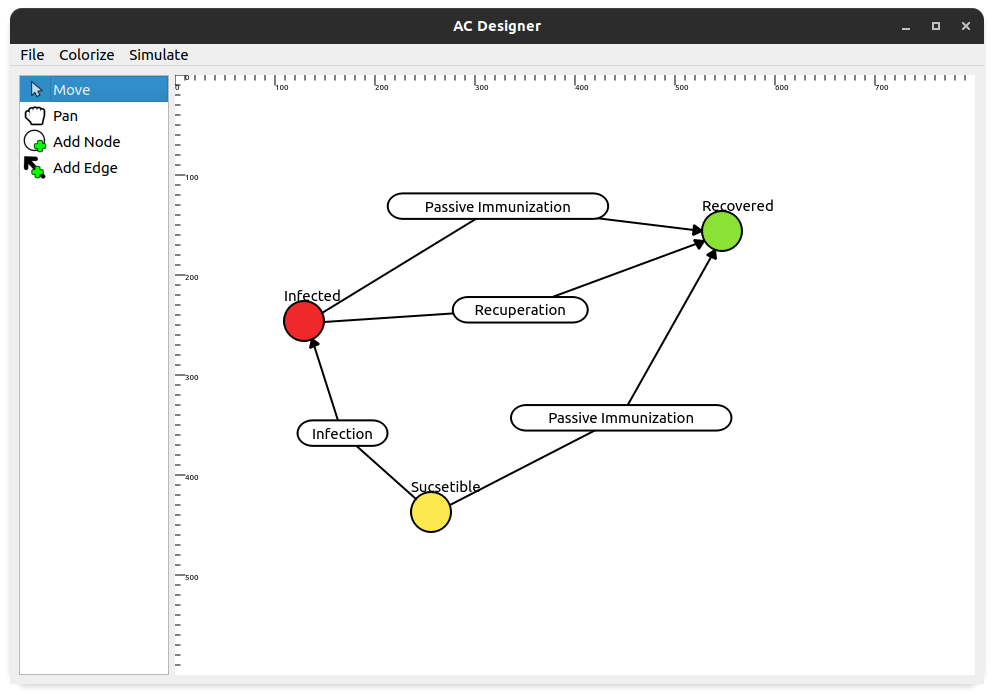
\includegraphics[width=.44\textwidth]{beamerthemesrc/images/ac-designer-sir.png}}}
        \quad
        \subfloat{{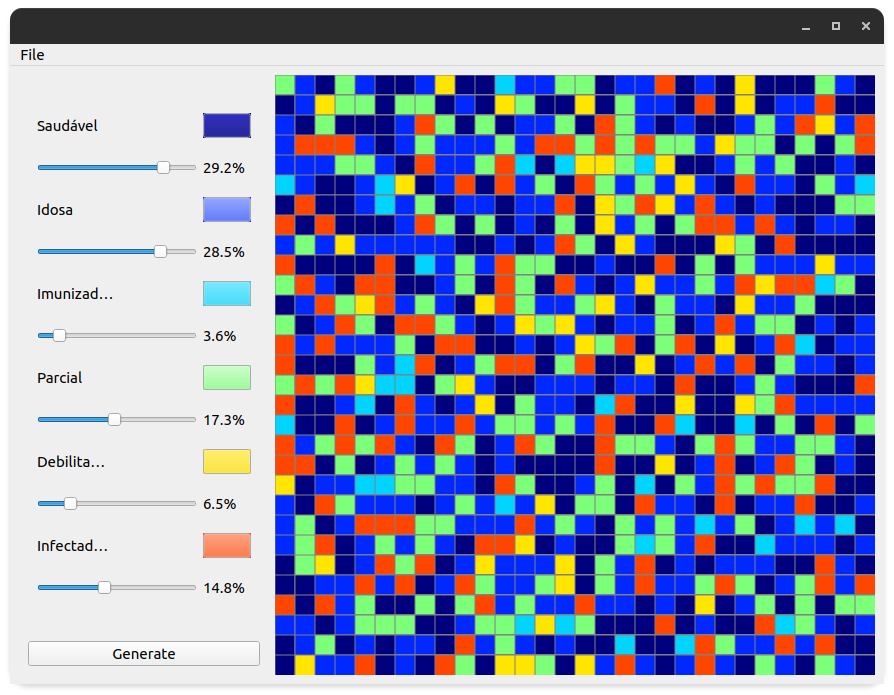
\includegraphics[width=.4\textwidth]{beamerthemesrc/images/ac-designer}}}
    
        \caption{Tela principal e de simulação do software.}
    \end{figure}
\end{frame}

\begin{frame}{Snoopy}
    \begin{itemize}
        \item Permite a modelagem de Redes de Petri;
        \item Utiliza uma representação baseada em grafos;
            \begin{itemize}
                \item Círculos representam estados (\textit{places}) e quadrados representam transições;
            \end{itemize}
        \item Foi uma grande inspiração às interfaces deste e do trabalho anterior, por ser simples de entender e representar;
        \item Assim como este trabalho, possui simulação \textit{onsite};
    \end{itemize}

    \begin{figure}
        \centering
    
        \subfloat{{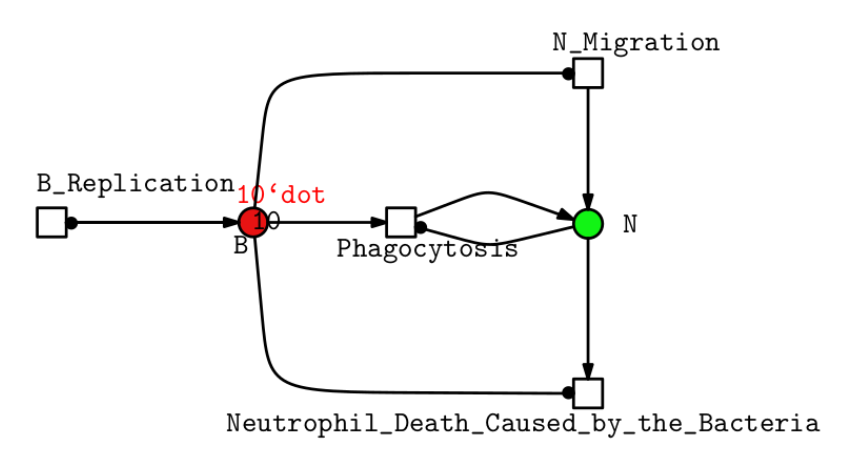
\includegraphics[width=.45\textwidth]{beamerthemesrc/images/snoopy-modelo.png}}}
        \quad
        \subfloat{{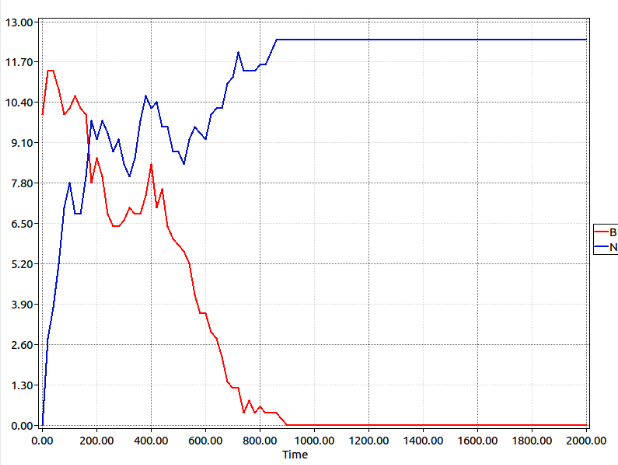
\includegraphics[width=.35\textwidth]{beamerthemesrc/images/snoopy-grafico.png}}}
    
        \caption{Exemplo de um modelo na interface e o resultado da simulação.}
    \end{figure}

\end{frame}

\begin{frame}{VCell e InsightMaker}

    \begin{columns}
        \begin{column}{.5\textwidth}
            \begin{itemize}
                \item O VCell é uma plataforma de modelagem de sistemas biológicos celulares;
                \item Os modelos são construídos com base em regras;
            \end{itemize}

            \begin{figure}
                \centering
                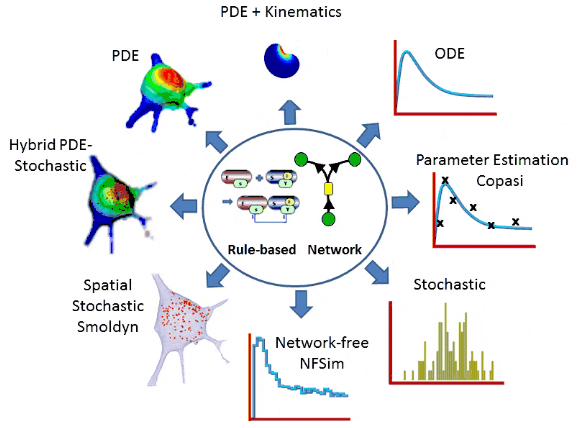
\includegraphics[width=.60\textwidth]{beamerthemesrc/images/vcell.png}
                \caption{Modelos suportados pelo VCell.}
            \end{figure}
        \end{column}

        \begin{column}{.5\textwidth}
            \begin{itemize}
                \item O InsightMaker permite a construção de modelos utilizando diagramas de Dinâmica de Sistemas e modelos baseados em agentes;
                \item Internamente, usa um modelo de EDOs;
            \end{itemize}

            \begin{figure}
                \centering
                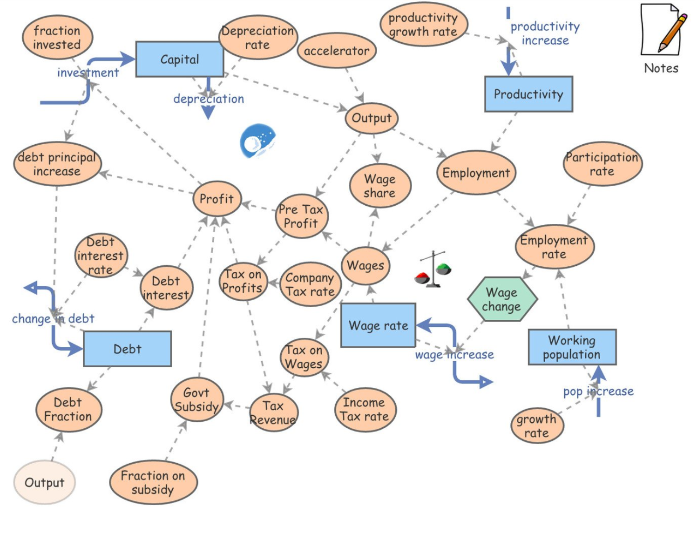
\includegraphics[width=.55\textwidth]{beamerthemesrc/images/insight-maker.png}
                \caption{Exemplo da GUI do InsightMaker.}
            \end{figure}
        \end{column}
    \end{columns}
\end{frame}
